\documentclass[10pt]{beamer}
\usepackage[utf8]{inputenc}
\usepackage[T1]{fontenc}
\usepackage{lmodern}
\usepackage{microtype}
\usepackage[]{amsmath}
\usepackage{accents}
\usepackage{amssymb}
\usepackage{amsfonts}
\usepackage{appendixnumberbeamer}
\usepackage[czech]{babel}
\usepackage[]{hyperref}
\usepackage{booktabs}
\usepackage{siunitx}
\usepackage[]{graphicx}
\usepackage[figurename=]{caption}
\usepackage[
    backend=biber
    ,style=iso-numeric
    ,autolang=other
    ,pagetotal=true
    ,sortlocale=cs_CZ
    ,bibencoding=UTF8
    ,spacecolon=false
    ,block=space
]{biblatex}
\addbibresource{citace.bib}

%\usetheme[sectionpage=none, numbering=fraction, progressbar= head, block=fill]{metropolis}
\usetheme[numbering=fraction, progressbar= head, block=fill]{metropolis}
\author{Michal Šesták}
\title{Multi-kompártmentový přístup ke kvantifikaci  objemové rychlosti přísunu zdrojů radonu do budov s využitím měřené intenzity větrání pomocí techniky indikačních plynů}
\subtitle{}
\institute{}
%\institute{Fakulta jaderná a fyzikálně inženýrská, ČVUT v Praze\\[0.5em]
%Vedoucí práce: Ing. Iva Ambrožová, Ph. D.}
\date{6. května 2019}
\begin{document}

\maketitle

%\begin{frame}{Obsah}
    %\tableofcontents
%\end{frame}
\begin{frame}{Osnova}
\item Úvod
\item Radon (Co to je, jeho dcery, proč je nebezpečný, co ovlivňuje jeho přísun do bytu, jak se měří, ochrana proti němu)
\item Rovnice
\item Model
\item Měření průtoků vzduchů
\end{frame}

\section{Radon (Co to je, jeho dcery, proč je nebezpečný, co ovlivňuje jeho přísun do bytu, jak se měří, ochrana proti němu)}

\begin{frame}[t]{Radon}
    \small
    \centering
    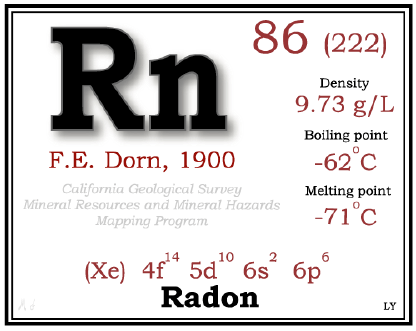
\includegraphics[width=.4\textwidth]{radon_overall.png}
    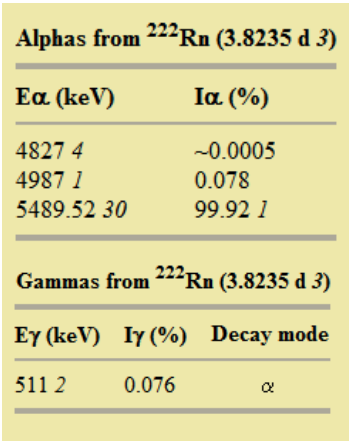
\includegraphics[width=.4\textwidth]{radon_decay.png}
    \cite{fronka}
\end{frame}

\begin{frame}{Radon}
    \small
    \centering
    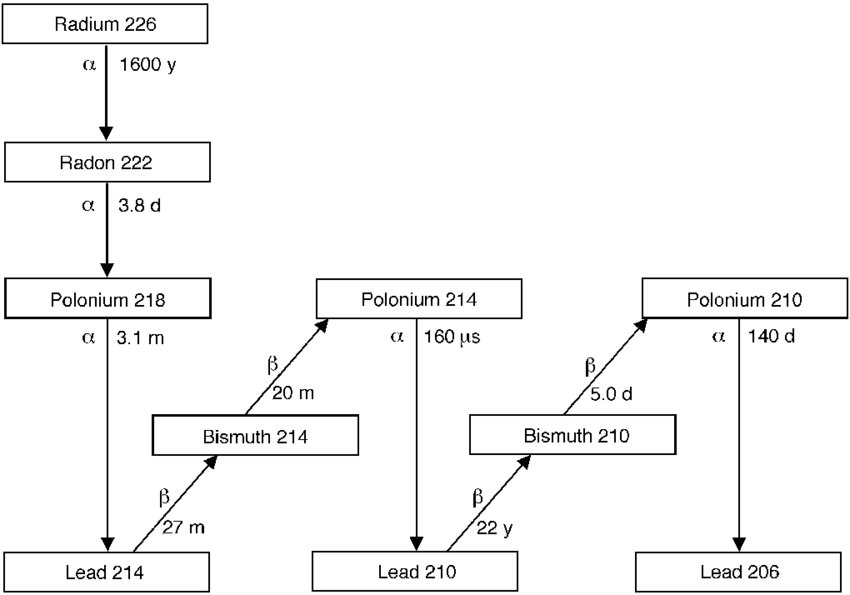
\includegraphics[width=.8\textwidth]{radon_chain.png}
\end{frame}

\begin{frame}{Hodnoty OAR pro různá prostředí}
    \small
    \centering
    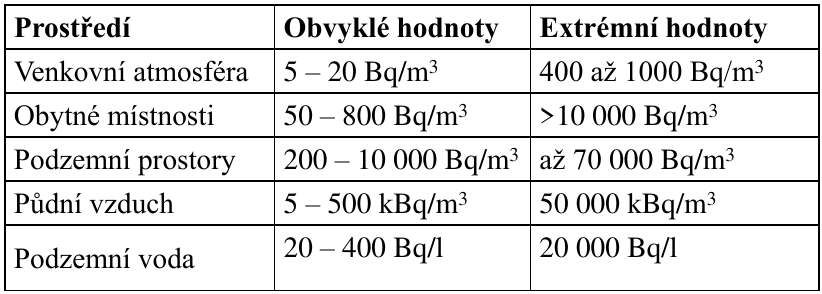
\includegraphics[width=.8\textwidth]{tabulka_hodnoty_radonu.png}
\end{frame}

\begin{frame}{Detektory radonu}
    \small
    dej sem dva obrazky -> stopace a radima
\end{frame}

\section{Můj výzkumný úkol}

\begin{frame}{Multi-kompártmentový přístup ke kvantifikaci  objemové rychlosti přísunu zdrojů radonu do budov s využitím měřené intenzity větrání pomocí techniky indikačních plynů}
    \small
    \centering
        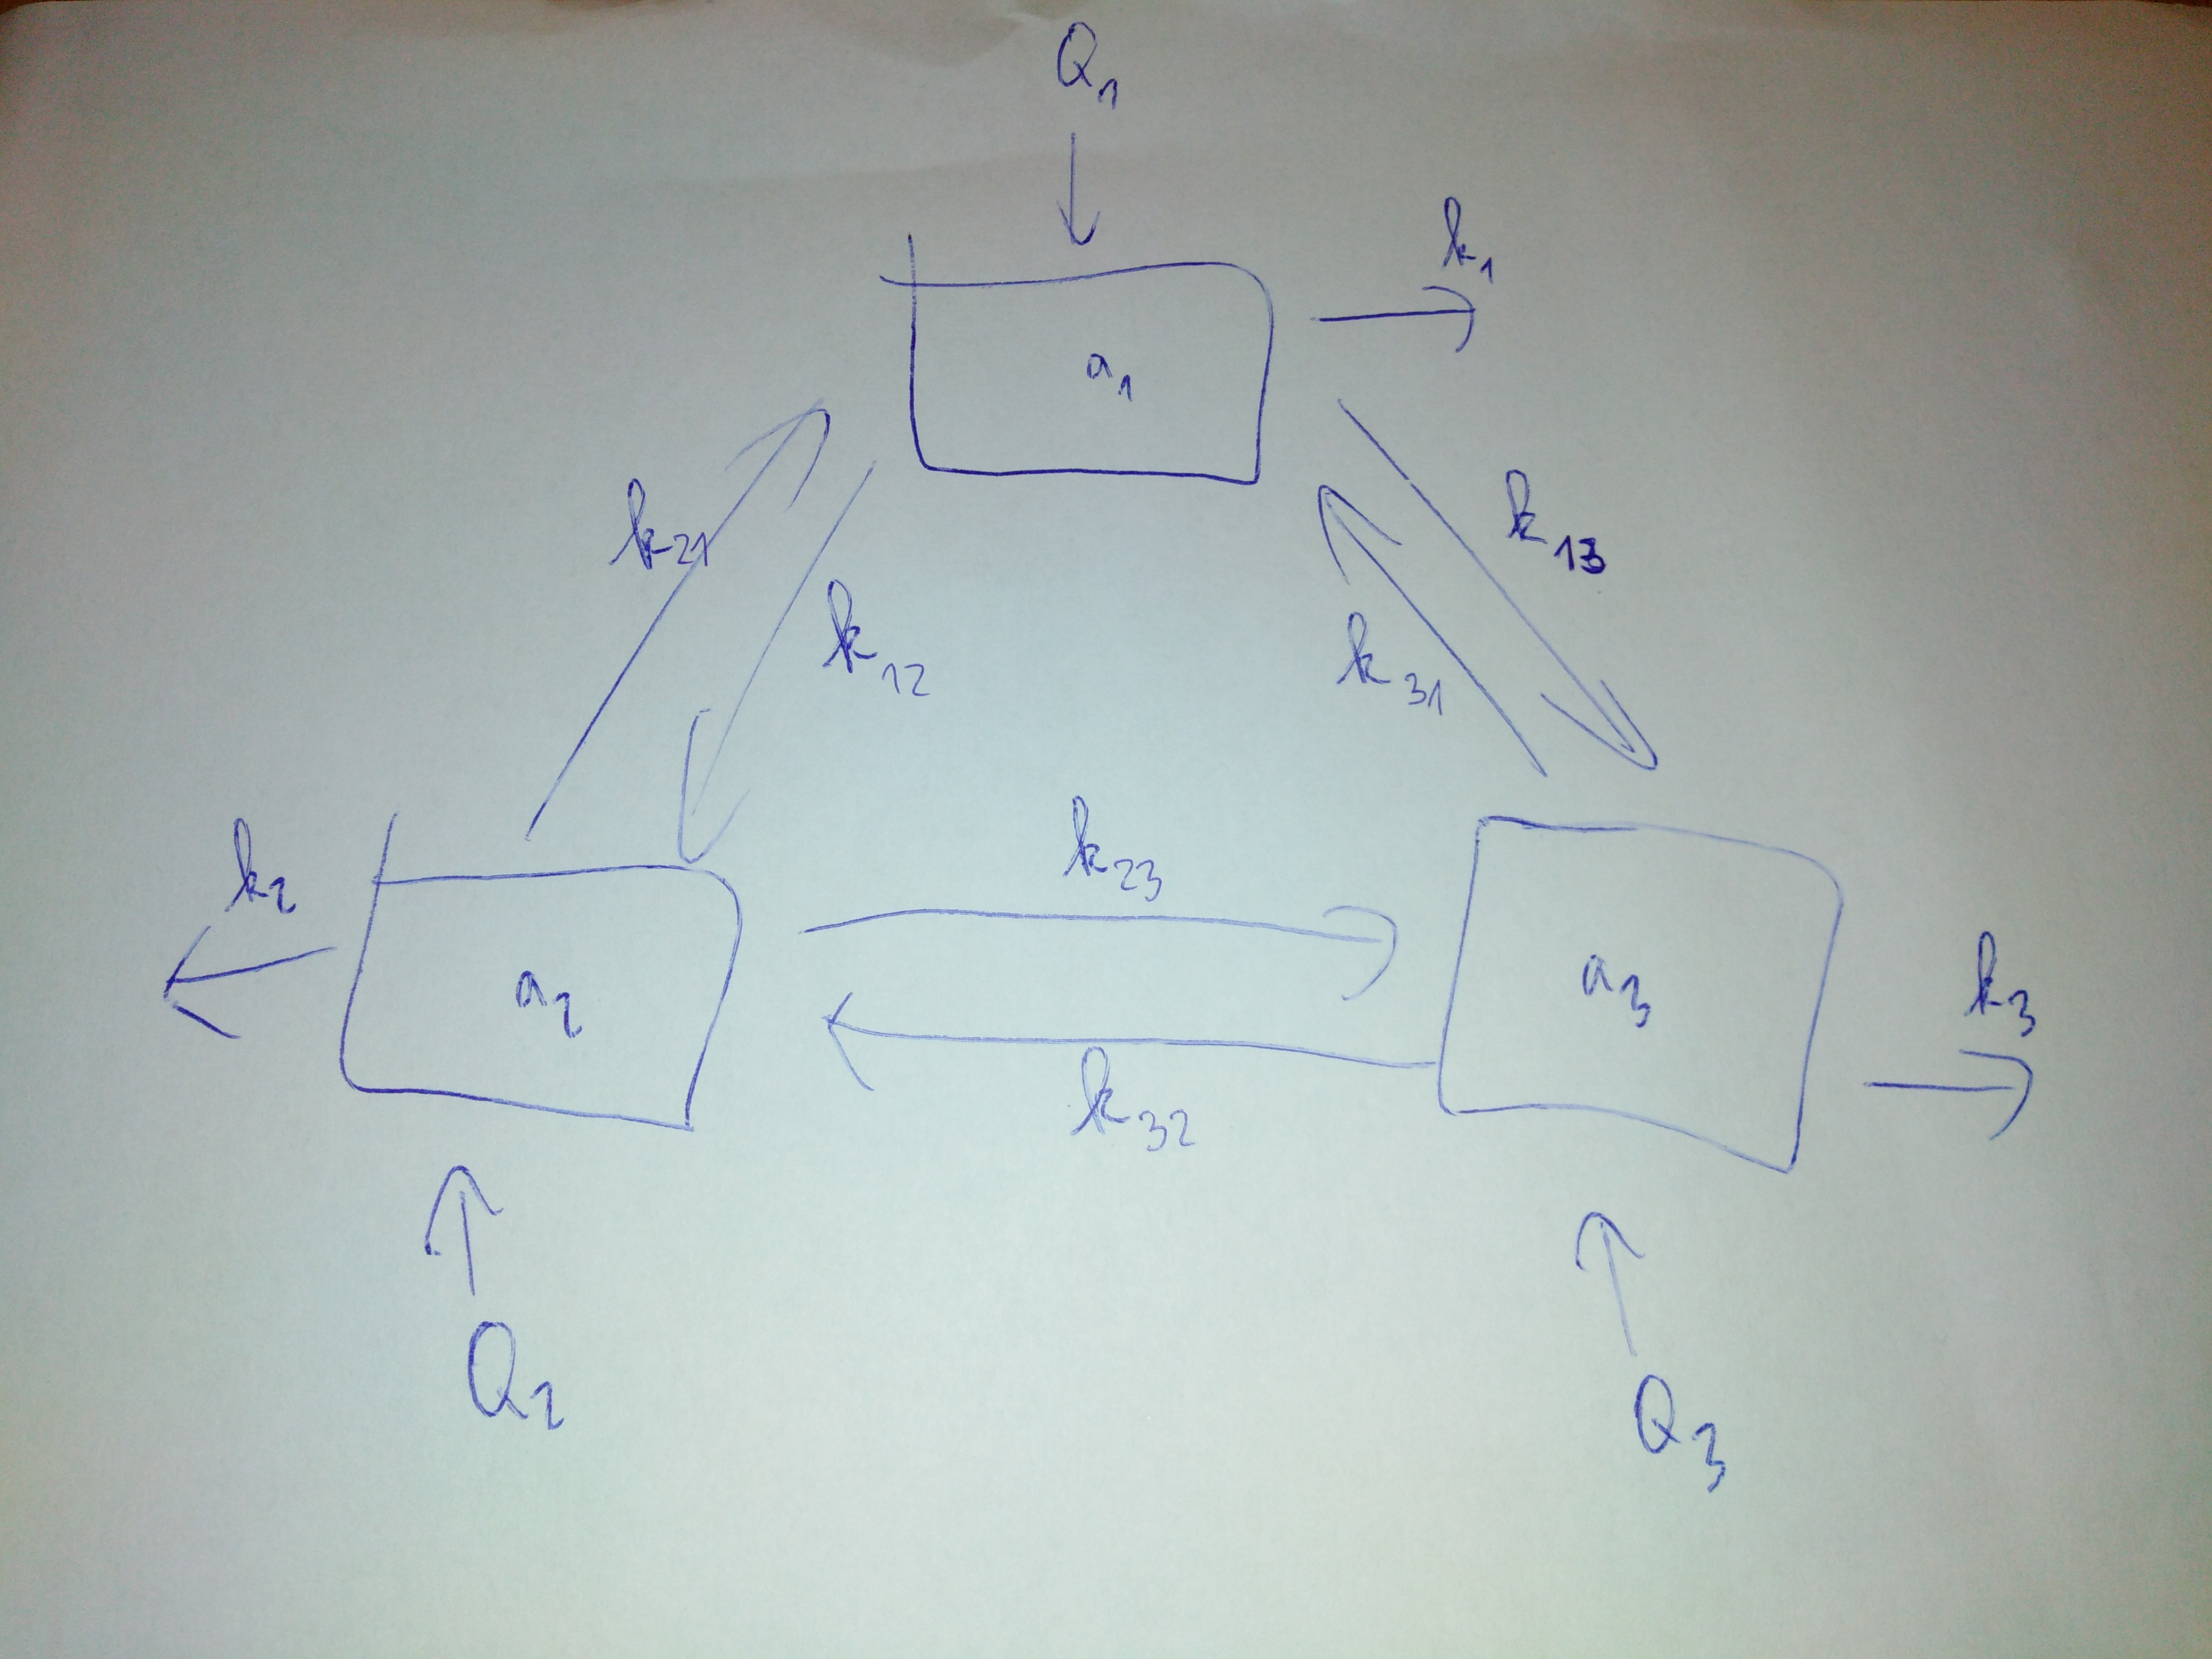
\includegraphics[width=.8\textwidth]{model.jpg}
\end{frame}

\begin{frame}{Model}
    \small
    \begin{equation}
        \dot{a_i}=\frac{1}{V_i}\left( \sum^n_{j=1}a_j k_{ji}-\sum^n_{j=1}a_i k_{ij}+Q_i \right)-(\lambda+k_i)a_i
        \label{eq:odvozovani}
    \end{equation}
        %\caption{<+Caption text+>}
        %\label{tab:<+label+>}
    \begin{table}
        \centering
        \begin{tabular}{lll}
            $a_i$ & koncentrace radonu v $i$-té zóně& [\si{Bq/m^3}] \\
            $V_i$ & objem $i$-té zóny& [\si{m^3}] \\
            $k_{ij}$ & objemový průtok vzduchu z $i$-té zóny do $j$-té zóny& [\si{m^3/hod}]\\
            $\lambda$ & přeměnová konstanta radonu& [\si{1/hod}]\\
            $k_i$ & výměna vzduchu $i$-té zóny& [\si{1/hod}] \\
            $Q_i$ & přísun radonu do $i$-té zóny& [\si{Bq/hod}] \\
        \end{tabular}
    \end{table}
\end{frame}

\begin{frame}{Model}
    \small
    \begin{align}
        V_i\dot{a_i}&=\sum^n_{j=1}a_j k_{ji}-\sum^n_{j=1}a_i k_{ij}-V_i(\lambda+k_i)a_i+Q_i\quad&\text{první varianta}\\
        V_i\dot{a_i}&=\sum^{n+1}_{j=1}a_j k_{ji}-\sum^{n+1}_{j=1}a_i k_{ij}-V_i\lambda a_i+Q_i\quad&\text{druhá varianta}
        \label{eq:rovnice}
    \end{align}
    \begin{itemize}
        \item druhá varianta v případě blízkosti uranových hald atd.
        \item \textbf{rovnovážný stav:}
            \begin{equation}
                0=\sum^n_{j=1}a_j k_{ji}-\sum^n_{j=1}a_i k_{ij}-V_i(\lambda+k_i)a_i+Q_i
            \end{equation}
    \end{itemize}
\end{frame}

\begin{frame}{Model - doplňující informace}
    \small
    \begin{itemize}
        \item Odhad nejistot $Q_i=Q_i(a_j, V_i, \dot{a_i}, k_{ij}, k_{ji}, k_i)$, $j\in\hat{n}$:
            \begin{equation}
                \sigma_{Q_i,Q_j}=\sum_k\sum_l\frac{\partial Q_i}{\partial x_k}\frac{\partial Q_j}{\partial x_l}\sigma_{x_k,x_l}\,,
                \label{eq:cov_matrix}
            \end{equation}
            ale není k dispozici výběrová kovarianční matice
        \item kontinuální měření: nahrazení derivace $\dot{a}$ diferencemi $\accentset{\circ}{a}_-, \accentset{\circ}{a}, \accentset{\circ}{a}_+$, např.:
            \begin{equation}
                \accentset{\circ}{a}=\frac{a(t+\tau)-a(t-\tau)}{2\tau}\,,
                \label{eq:centralni_diference}
            \end{equation}
            $\tau=\SI{30}{min}$ je časový krok
    \end{itemize}
\end{frame}

\begin{frame}{Měření průtoků vzduchu mezi zónami}
    \small
    \begin{itemize}
        \item indikační plyny = perfluorokarbony,
            \begin{itemize}
                \item netoxické, inertní, čisté, bezbarvé, nehořlavé a neradioaktivní plyny. 
                \item v přírodě se nevyskytují
            \end{itemize}
        \item $N$ zón = minimálně $N$ tracerů
        \item vyvíječe
        \item integrální detektory, analýza tracerů pomocí chromatografie
        \item další instrumentace: laserové dálkometry, kontinuální měřidla teploty, dávkovače tracerů do vyvíječů, pinzety atd.
        \item \textbf{doba měření}: 7 dní (screening) nebo jeden měsíc v běžném uživatelském režimu
            
    \end{itemize}
\end{frame}

\begin{frame}{Detektory a vyvíječe}
    \small
        \centering
        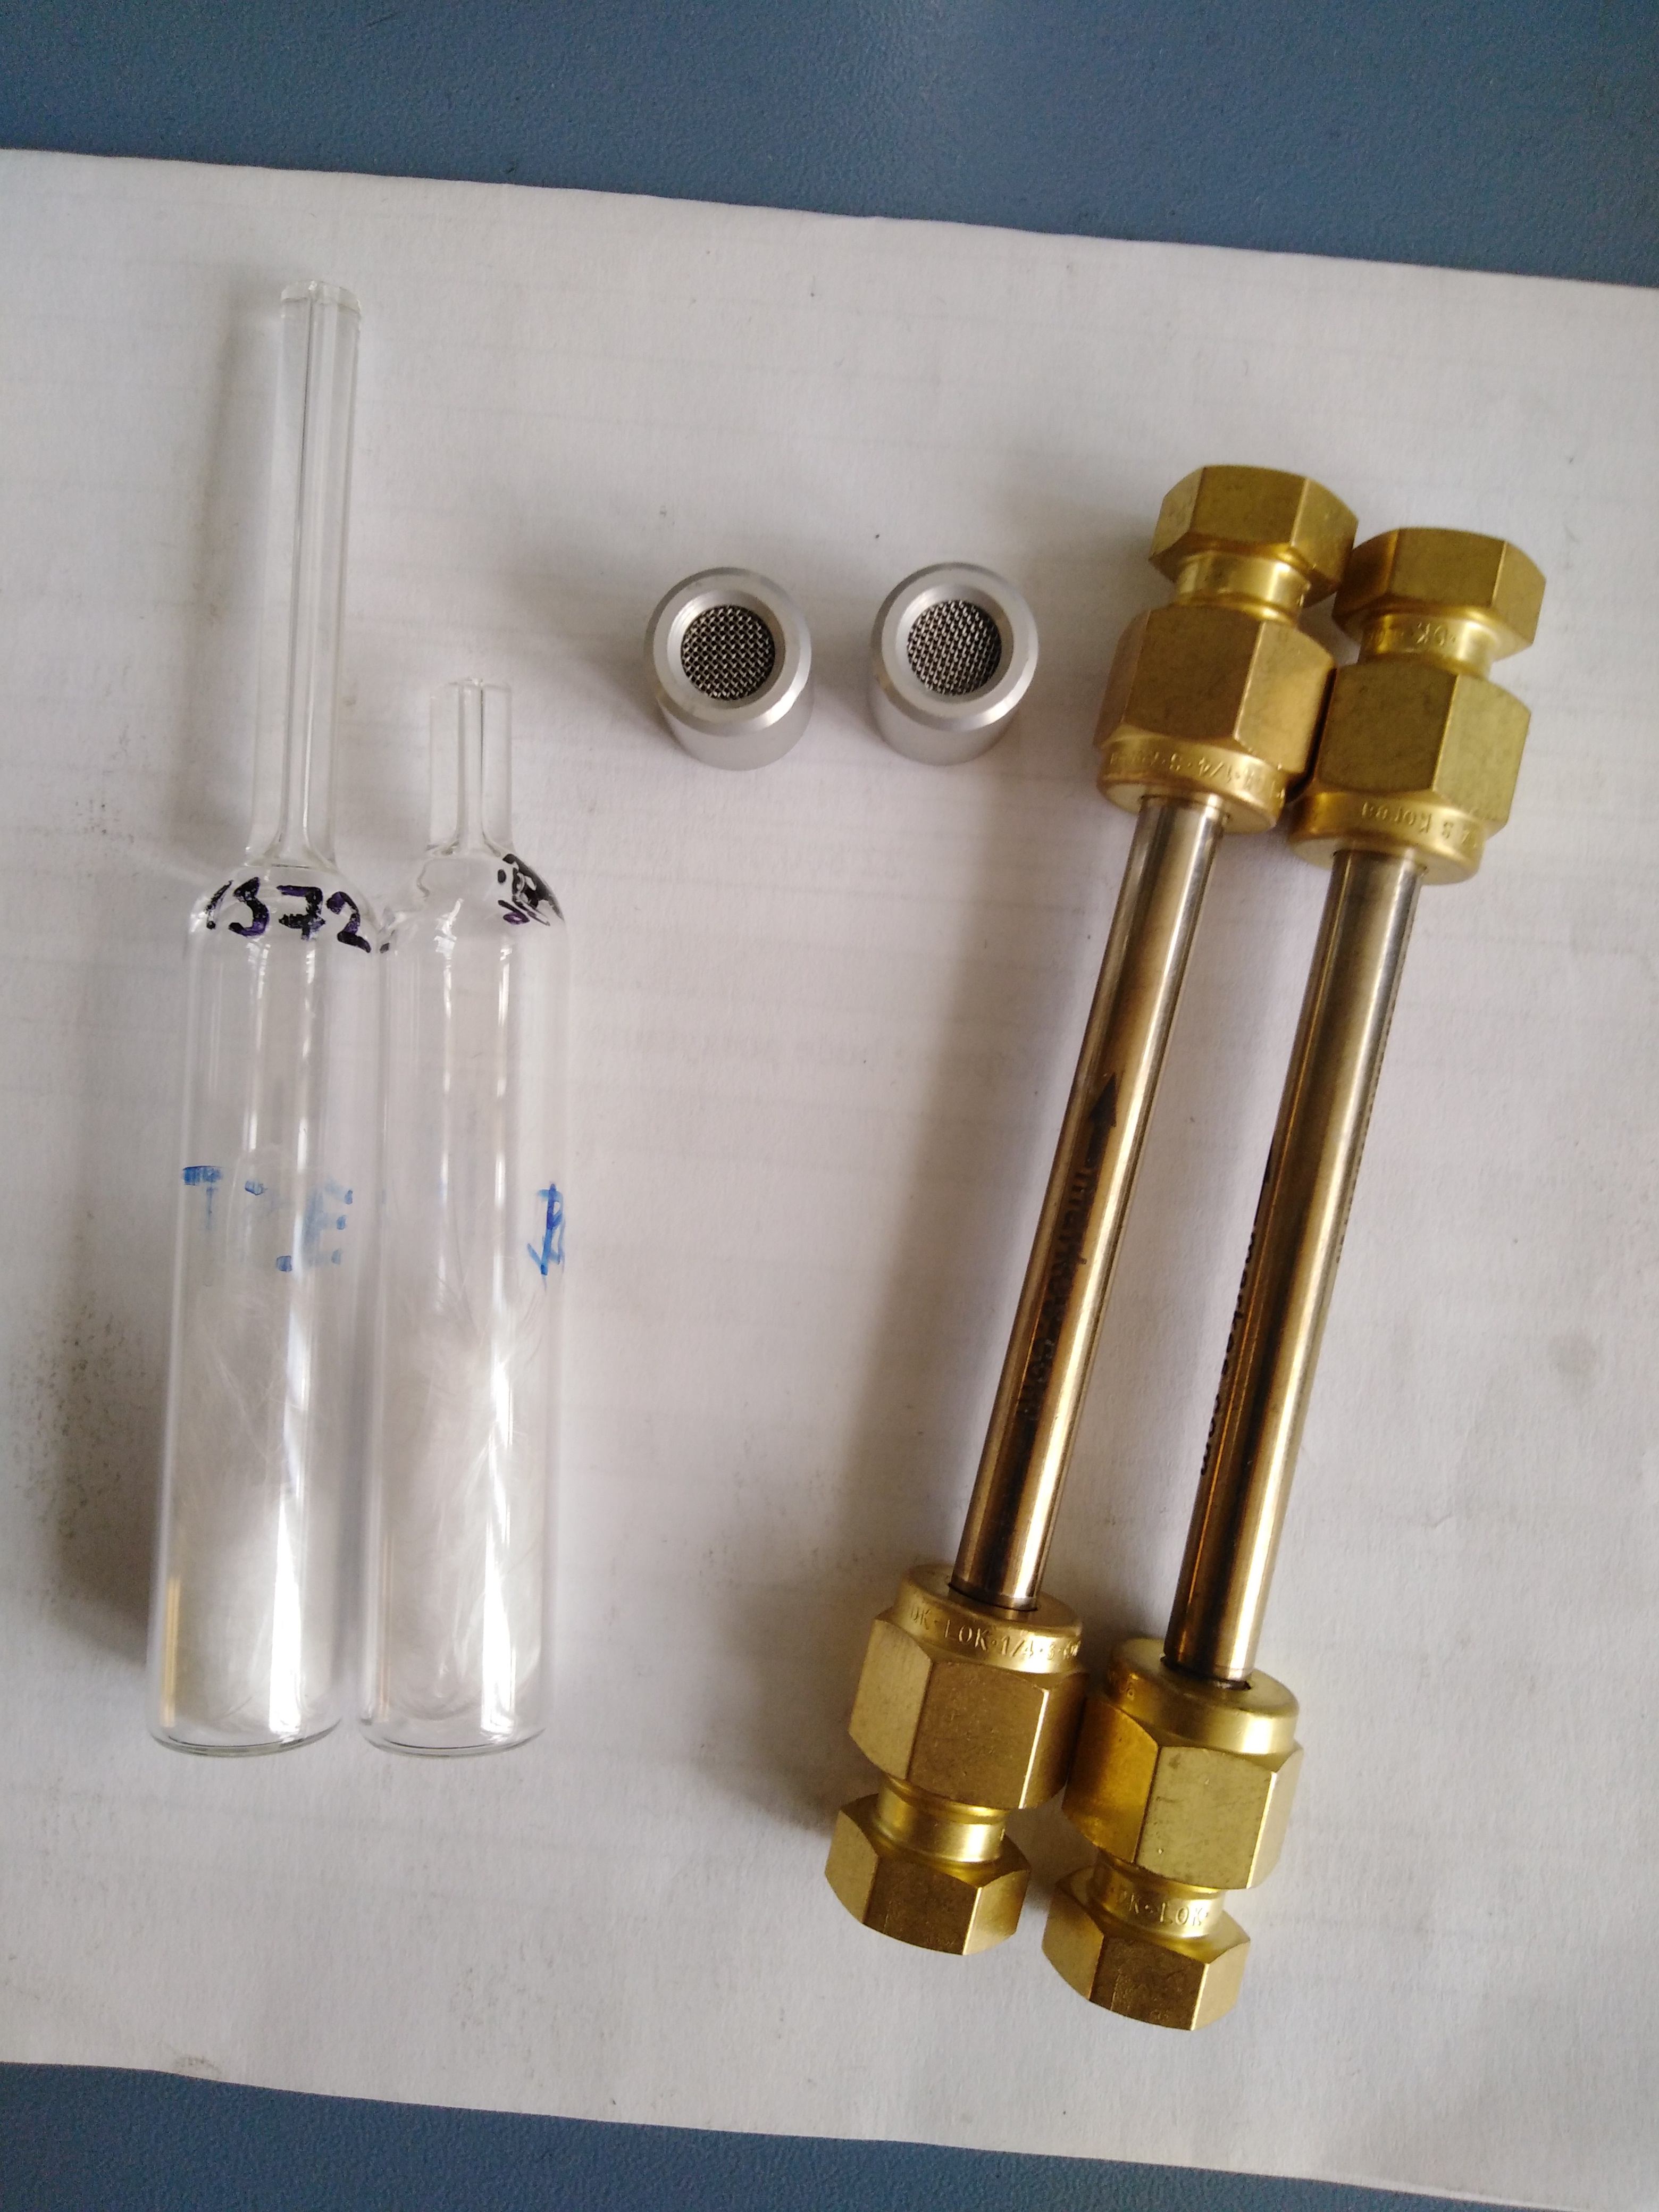
\includegraphics[width=.45\textwidth]{1.jpg}
        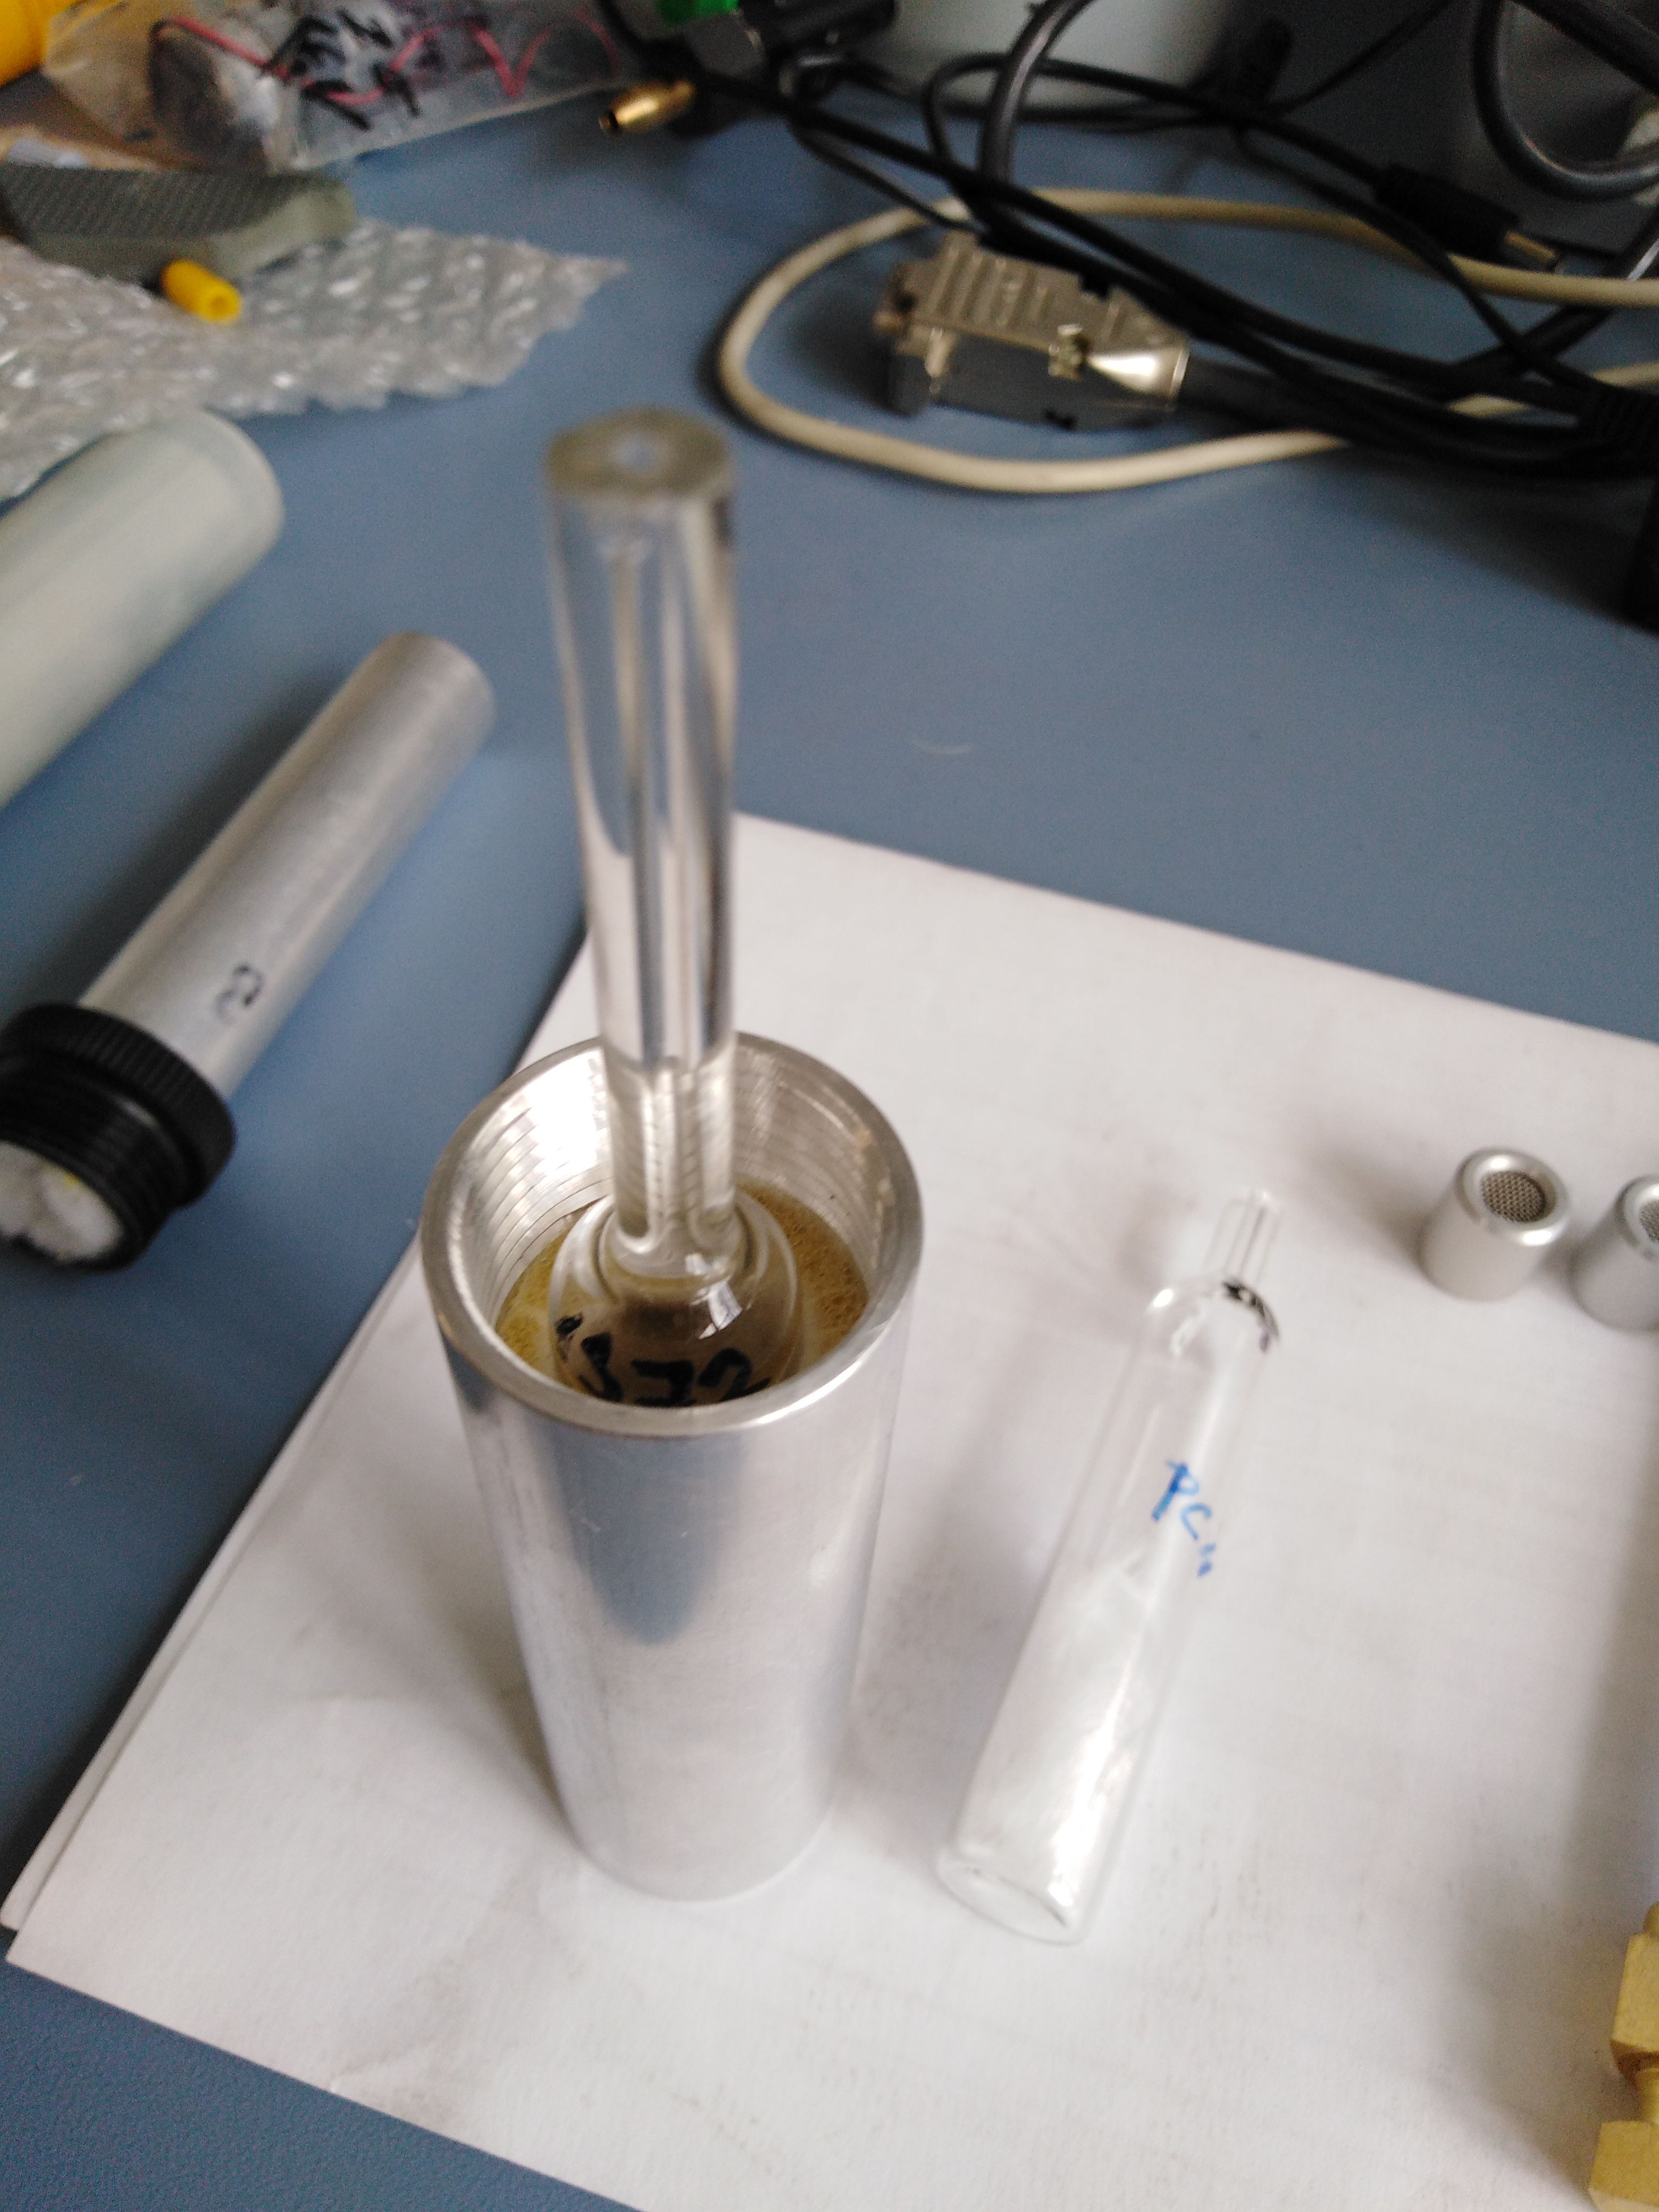
\includegraphics[width=.45\textwidth]{3.jpg}
\end{frame}

\begin{frame}{Dávkovač}
    \small
    \centering
        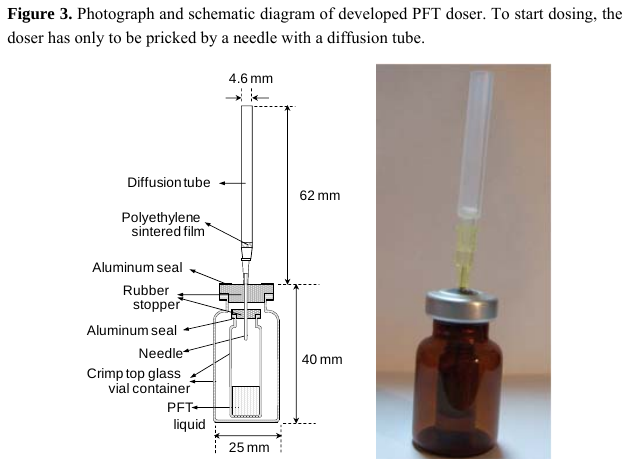
\includegraphics[width=.7\textwidth]{davkovac.png}
        \cite{japonci2}       
\end{frame}

\begin{frame}{Detektor}
    \small
    \centering
        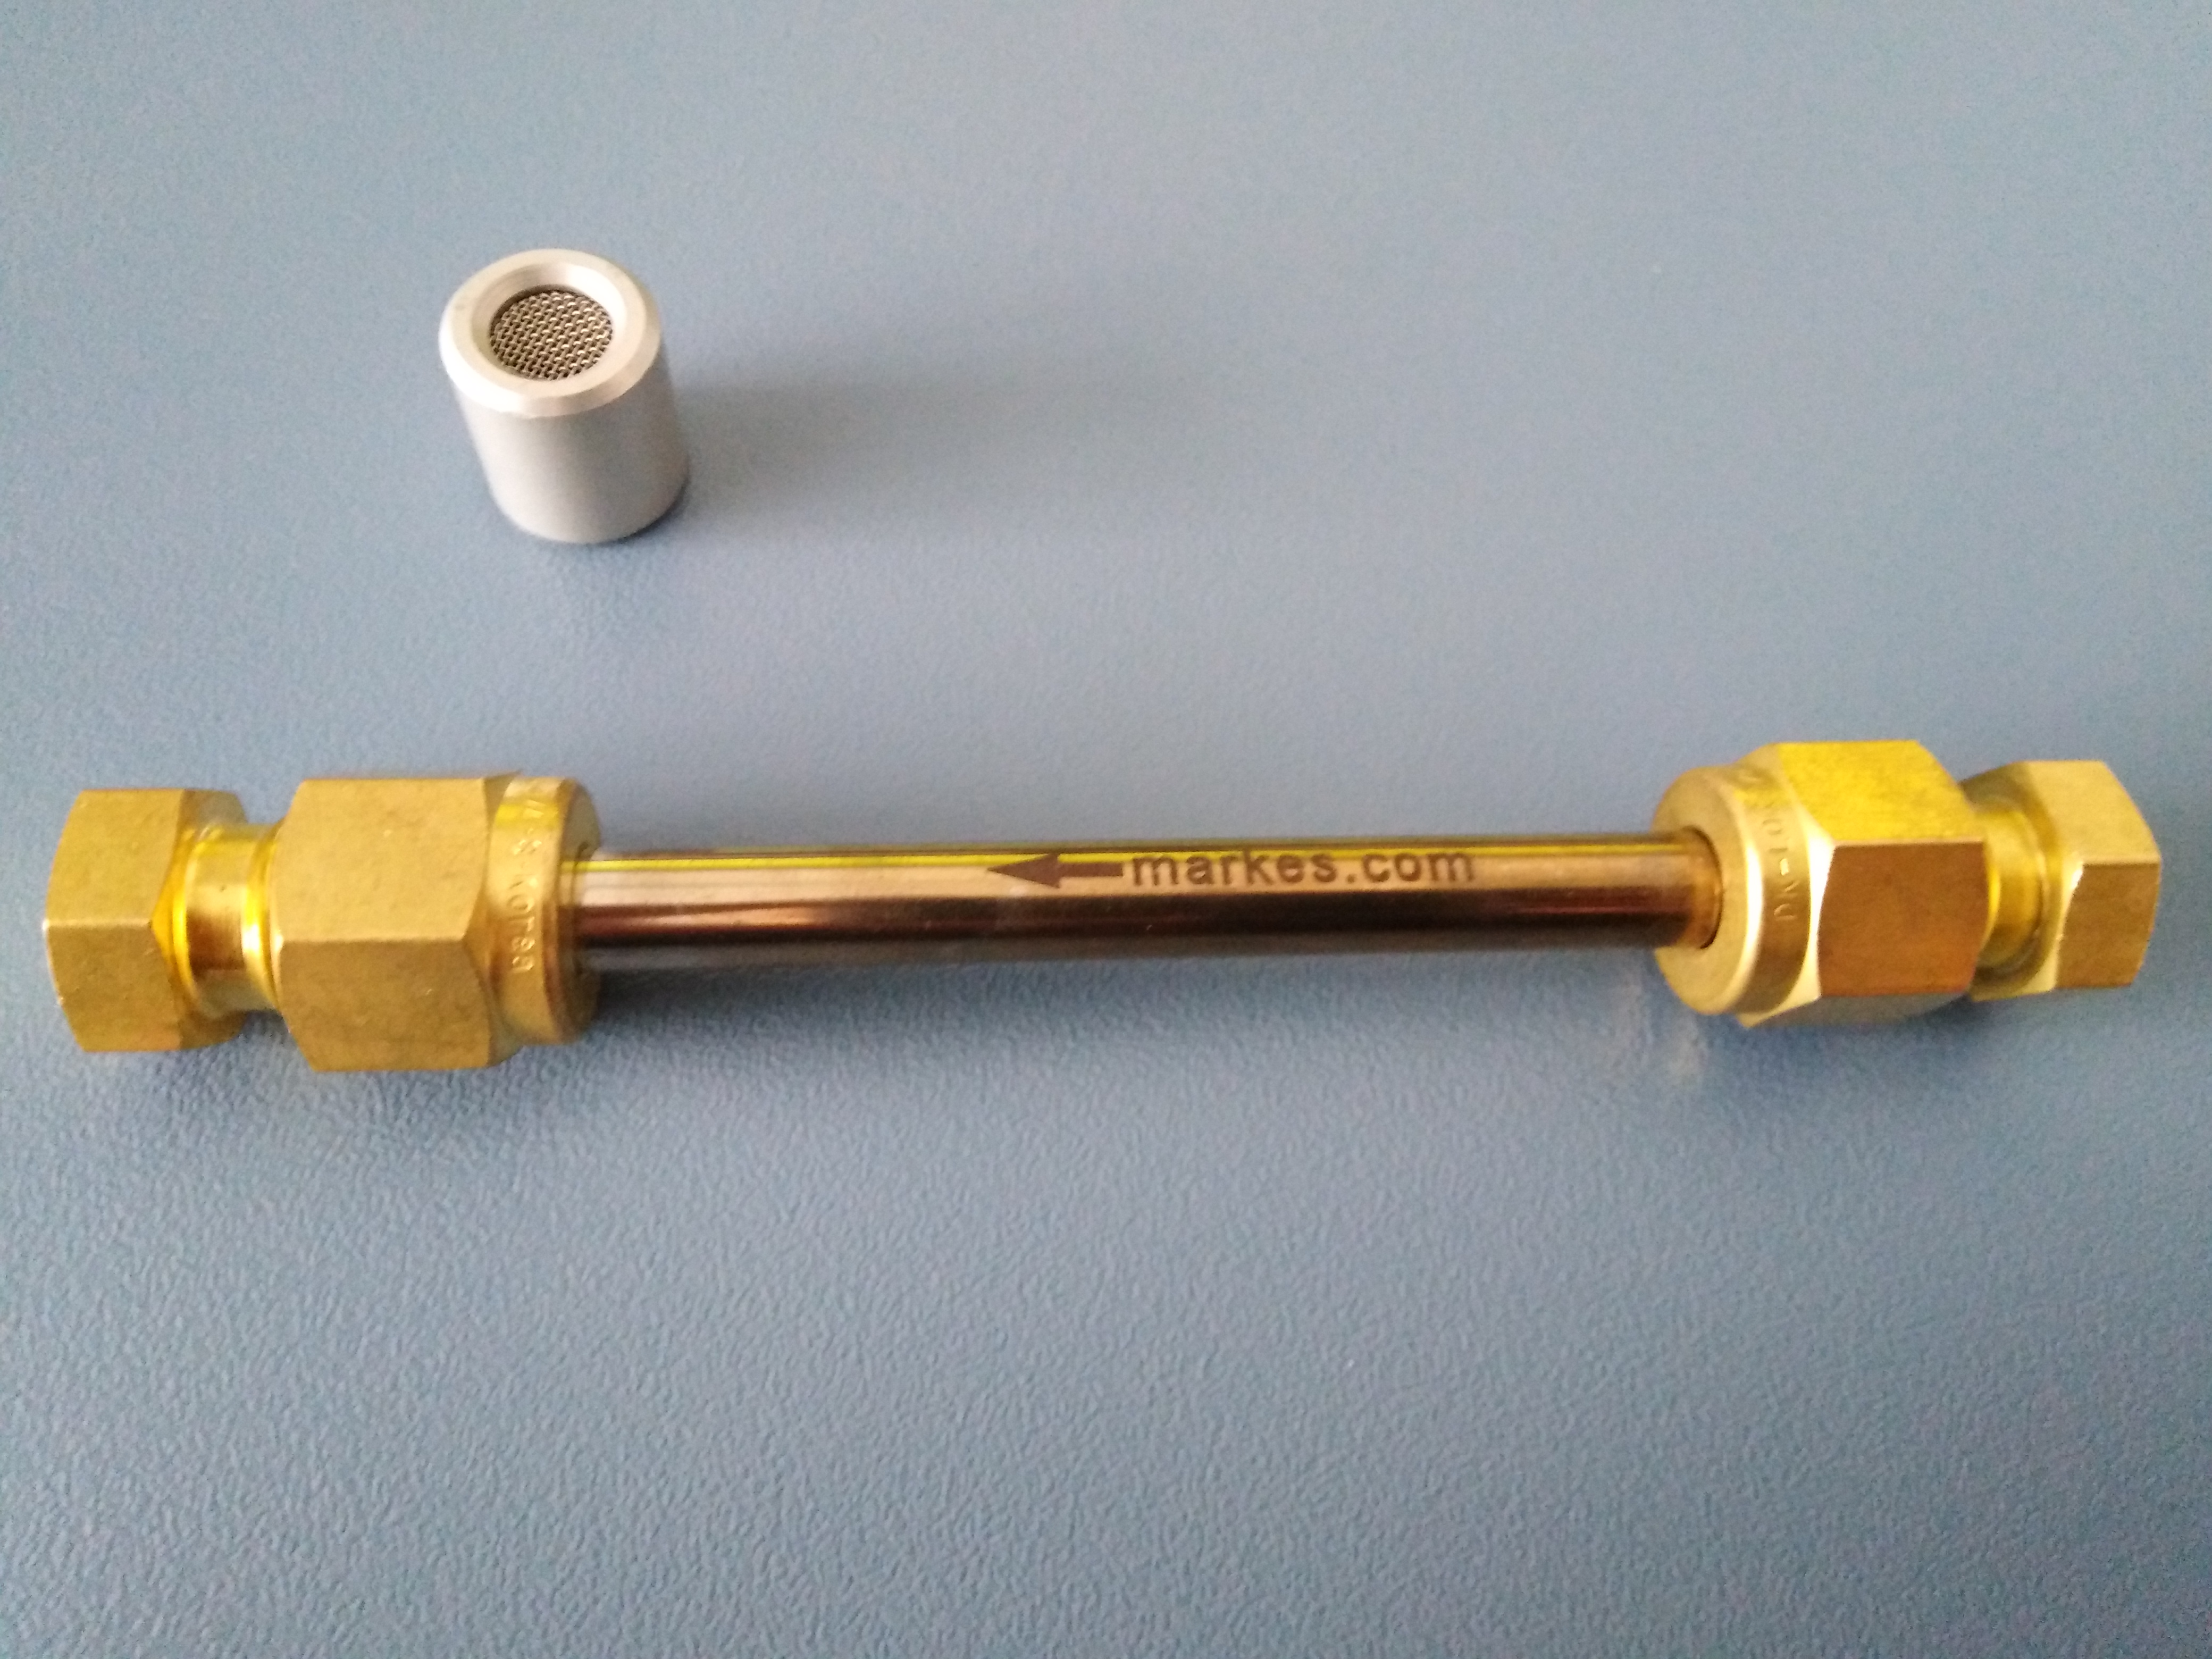
\includegraphics[width=.6\textwidth]{meridlo_traceru.jpg}
\end{frame}

\begin{frame}{Modelový příklad 1}
        \centering
        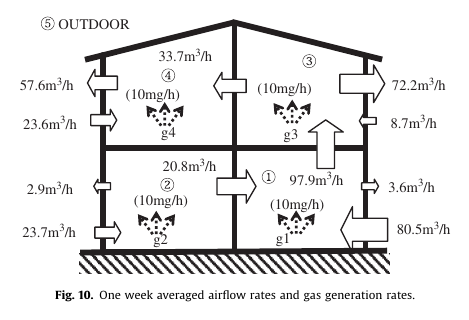
\includegraphics[width=.9\textwidth]{zony.png}
        \cite{japonci}       
\end{frame}

\begin{frame}{Modelový příklad 2}
        \centering
        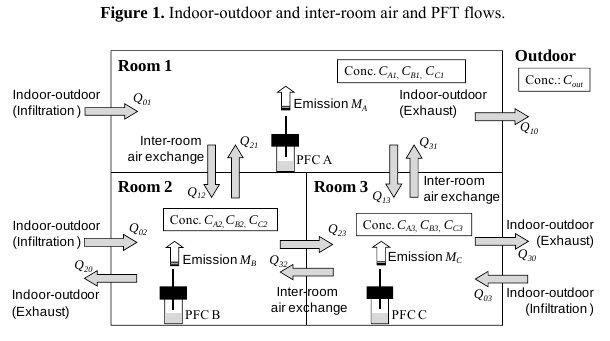
\includegraphics[width=.9\textwidth]{zony2.png}
        \cite{japonci2}       
\end{frame}

\begin{frame}{Problémy}
    \small
    \begin{itemize}
        \item nehomogenita koncentrace indikačních plynů v jednotlivých zónách => rozdělení na podzóny, použití pravděpodobnostních distribucí
        \item mohou vycházet záporné průtoky/výměny vzduchu -> je nutná kvalitní analýza nejistot
    \end{itemize}
\end{frame}

% různá nastavení
%\metroset{sectionpage=simple,none}
%\begin{overlayarea}{\textwidth}{\textheight}\end{overlayarea}


\begin{frame}[allowframebreaks]
    \nocite{*}
\renewcommand*{\bibfont}{\tiny}
\printbibliography
\end{frame}
\end{document}
